\chapter{Activity Lifecycle}
\label{ALI:ALII}

\section{Introduction}
...To be filled...

\section{Activity Basics}
\label{ALI:activityBasics}

You can think of an ``\href{https://developer.android.com/guide/components/activities.html}{\texttt{Activity}}'' as a screen (this concept was also briefly introduced in section \ref{TOAS:activity}). Imagine an application in which you can navigate from one screen to another screen, such as home to settings screen. Ideally for each screen there would be one activity responsible for displaying its layout and running its logic. There can be as many screens or activities in an android app as required.

Each activity consists of exactly one java file and zero or more layout files. Yes there can be an activity that doesn't have any layout at all e.g: an activity running in the background! 

When ever you create a new ``Empty'' project, one activity is created by default having ``\texttt{MainActivity.java}'' and ``\texttt{activity\_main.xml}'' files attached to it. When you run the app you will see only one screen displaying ``Hello World!'' text. Rest of the chapter discusses activities in more detail. 

\section{Lifecycle Callbacks}
\label{ALI:lifecycleCallbacks}

As mentioned above there can be many activities in an android app but \textit{only one} activity is active at any given time. From its birth to death every single activity under goes a series of stages. When you tap the app icon on your phone's home screen it launches that app. Then there is a period when the app is being loaded in the memory. After this there is a period when the app is fully loaded but hasn't yet displayed on the screen. The next stage is when the app is ready and is displayed on the screen. Similar stages occur when the app is destroyed.

For each stage android notifies the activity through callback methods. Following figure shows complete lifecycle of an app along with their callback methods \textit{(image source: \href{https://developer.android.com/images/training/basics/basic-lifecycle.png}{android developer portal})}:

\begin{center}
	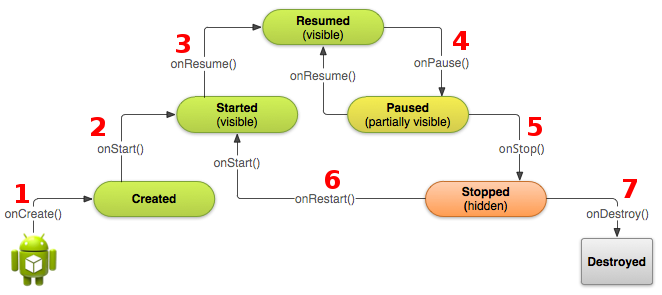
\includegraphics[scale=0.5]{chapters/ch08/images/1}
\end{center}

There are essentially seven states an activity can be in, as labeled in the above figure. Let's take a look at these one by one:

\begin{enumerate}
	\item \texttt{onCreate()}: This is the only method in the activity lifecycle that MUST be implemented. All other methods are optional. \texttt{onCreate()} method is called when the operating system is loading the activity into the memory. This is a good place to do heavy duty initialization that takes many seconds or even minutes to complete. For example you could load the layout here (which is already being done in the default code), or you could load data bases here.
	
	\textbf{\underline{Important:}} This method will also be called when the device changes its orientation from portrait to landscape and vice versa. 
	
	\item \texttt{onStart()}: This method is called when the activity is fully loaded in the memory and now in the process of being displayed on the screen. Here you can do very light initialization such as resetting variables or resuming any sounds and animation effects. Note that the activity is partially visible on the screen. This method is quickly followed by \texttt{onResume}.
	
	\item \texttt{onResume()}: Called when the activity is fully visible and completely active. The user can now interact with the activity until it loses focus again.
	
	\item \texttt{onPause()}: This method is called when the activity is \textit{``partially''} visible i.e: it is obstructed by some other foreground activity such as a dialog box or a floating fragment. 
	
	\item \texttt{onStop()}: The \texttt{onStop} method is called when the activity goes into background or is \textit{``fully''} hidden e.g by another activity. Note that this method will also be called when the user presses the home on his device to send the running app into background. This is a good place to de-allocate all the resources that were created in the \texttt{onStart} method.
	
	\item \texttt{onRestart()}: When an activity is brought focus from a stopped state the \texttt{onRestart()} method is called. For example the user switches from some other app to this app, or unloads some activity that was loaded from the current activity. So when this method is called you know for sure that an already running activity is being brought back to life again.
	
	\item \texttt{onDestroy()}: This method is called when the activity is being completely destroyed from the memory. Unlike other lifecycle methods, this method is \textbf{NOT} guaranteed to be called. For instance if the user gracefully exits the activity this method will be called. On the other hand if for any reason the operating system violently terminates the activity then this method will NOT be called. \textit{Since this method is not guaranteed to be called, you should not rely on it and should not save or de-allocate resources in it}. 
	
\end{enumerate}

\begin{quotation}
	\textit{``\texttt{\underline{Note}}: An activity can go from one state to another state IF and ONLY IF there is a link between these states, and this link is `directional'. For example referring to the above figure, any activity can go from \texttt{Started} state to \texttt{Resumed} state; but it CANNOT go directly from \texttt{Resumed} to \texttt{Stopped}, it has to go through the texttt{Paused} state.''}
\end{quotation}

Let's create a new project that will be used in this chapter.

\subsection{Create a New Project}
\label{ALI:createProj}

Create a new project from scratch. Perform the following steps:
\begin{enumerate}
	\item Create a new project having name ``\texttt{Ch\ref{ALI:ALII}}''
	\item Select minimum API 16 : Android 4.1 (Jelly Bean).
	\item Select ``\texttt{Empty Activity}''
	\item Accept default values for activity and click finish. \\
\end{enumerate}

\subsection{Implementing Activity Lifecycle Methods}
Open up \texttt{MainActivity.java} and add the following lifecycle methods as shown below:

\begin{center}
	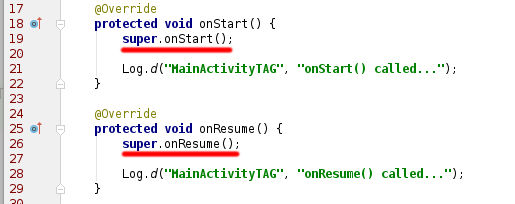
\includegraphics[scale=0.4]{chapters/ch08/images/2}
\end{center}

We just implemented the two methods namely \texttt{onStart} and \texttt{onResume}. Specially note lines numbered 19 and 26 (underlined with red). 

\begin{quote}
	\textit{``It is extremely important to call the same super class (base class) methods at the beginning of each activity lifecycle method.''}
\end{quote}

\subsubsection{Exercise:}
Implement all of the activity lifecycle methods discussed above. In each method you can either display messages through \texttt{Log.d} as done above OR through \texttt{Toast}.

\subsection{Lifecycle Methods in Action}
Assuming that you've implemented all seven of the lifecycle methods. Let's see them in action. Add another activity by going to ``File $\rightarrow$ New $\rightarrow$ Activity'' and select ``Empty Activity''. Configure activity dialog box will appear. Enter the activity name as ``\texttt{SecondActivity}'', layout name will change automatically. Accept other entries as default and hit finish:

\begin{center}
	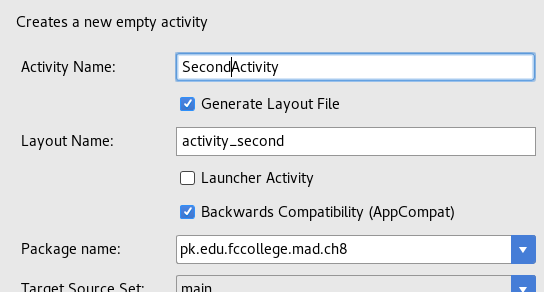
\includegraphics[scale=0.4]{chapters/ch08/images/3}
\end{center}

After you've completed the above process a new activity will be created by the android studio having \texttt{SecondActivity.java} and \texttt{activity\_second.xml} files attached to it:

\begin{center}
	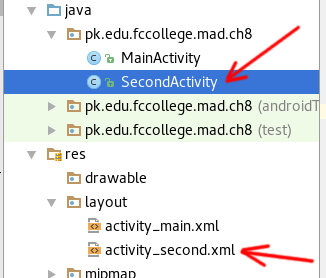
\includegraphics[scale=0.4]{chapters/ch08/images/4}
\end{center}

If you open up ``\texttt{AndroidManifest.xml}'' you'll notice that the new activity we just created is now added to this file (line 18):

\begin{center}
	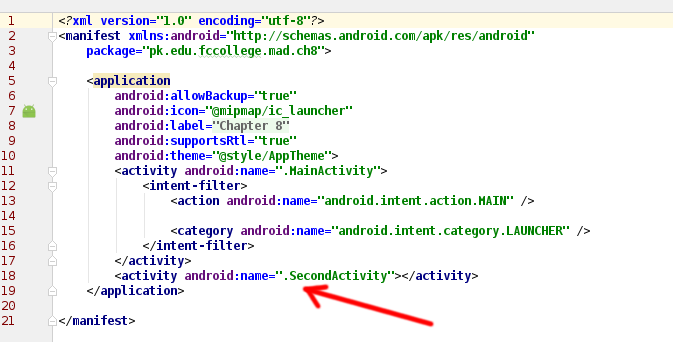
\includegraphics[scale=0.4]{chapters/ch08/images/5}
\end{center}

``\textbf{Note:} All activities must be listed in the Android Manifest file. The android studio does this automatically when you create a new activity through the wizard. Otherwise you need to add this manually if you are creating the activity by creating java and layout files separately and independently. The dot `\texttt{.}' you see in `\texttt{.SecondActivity}' above is a short hand for mentioning the entire package name i.e: \texttt{pk.edu.fccollege.mad.ch8.SecondActivity}''. \\

Open up \texttt{activity\_second.xml} and make its layout as follows (it just contains a bit centered text view label):

\begin{center}
	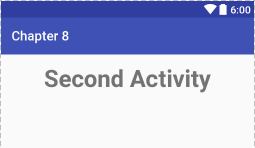
\includegraphics[scale=0.4]{chapters/ch08/images/6}
\end{center}

Now open up \texttt{activity\_main.xml} and add a button, name it anything you want. For this chapter we name it ``Submit''. Try to match its layout with the following. Add some space between the text label and the button, we will need it shortly: 

\begin{center}
	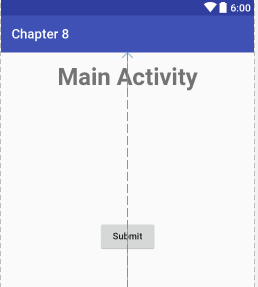
\includegraphics[scale=0.4]{chapters/ch08/images/7}
\end{center}

After that attach an event listener named \texttt{onBtnClicked} to this button. The listener should reside in \texttt{MainActivity.java}. Add the following code in this method:

\begin{center}
	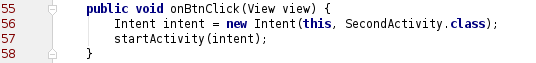
\includegraphics[scale=0.4]{chapters/ch08/images/8}
\end{center}

\begin{itemize}
	\item \textit{Line 56:} Create an intent object (more details about intents are given in a future section \ref{ALI:explicitIntents}). Initialize the intent object with the name of the \texttt{SecondActivity} class.
	
	\item \textit{Line 57:} \texttt{startActivity} method will launch the second activity.
\end{itemize}

If you run this app on a device and look into the ``LogCat'' output, you will see the following messages as \texttt{MainActivity} is displayed on the screen:

\begin{center}
	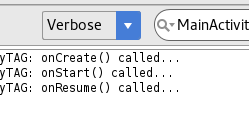
\includegraphics[scale=0.4]{chapters/ch08/images/9}
\end{center}

This is expected as we saw in the activity lifecycle diagram in section \ref{ALI:lifecycleCallbacks}. Now press the ``Submit'' button on the main activity, this will launch the Second Activity and send main activity to the background. If you look at the logcat window you will see other lifecycle methods being called:

\begin{center}
	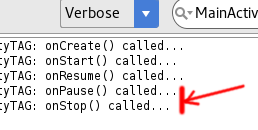
\includegraphics[scale=0.4]{chapters/ch08/images/10}
\end{center}

From the second activity if you press the back button, the current activity will be removed and main activity will be brought back to life again, calling the following lifecycle methods as expected:

\begin{center}
	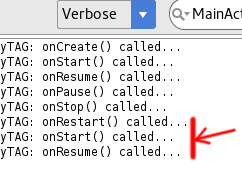
\includegraphics[scale=0.4]{chapters/ch08/images/11}
\end{center}

With the main activity on the screen, when you press the back button the \texttt{onPause}, \texttt{onStop} and \texttt{onDestroy} methods will be called in sequence and the app will be gracefully removed from the system resources:

\begin{center}
	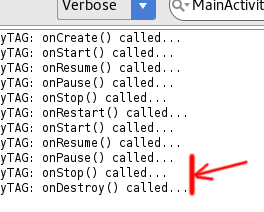
\includegraphics[scale=0.4]{chapters/ch08/images/12}
\end{center}

\begin{quote}
	\textit{\textbf{Note:} If you or the system forcefully terminates the app, then only \texttt{onPause} and \texttt{onStop} will be called. \texttt{onDestroy} will \textbf{NOT} be called.}
\end{quote}

Let's explore the pause state a bit more. Pause state occurs when the activity is partially visible, obstructed by another activity or is in the transition of going into the background. Right now this happens so fast that the \texttt{onStop} is followed by \texttt{onPause} without any delay. Let's fix this. \\

Open up \texttt{styles.xml} and add an \texttt{<item>} element having \texttt{name} attribute as \texttt{android:windowIsFloating} and set it to true as show below (line 9):

\begin{center}
	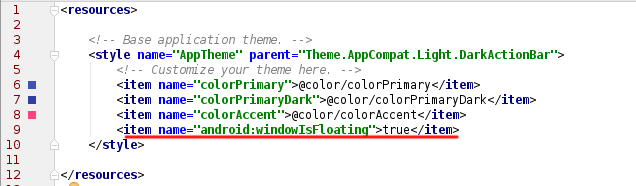
\includegraphics[scale=0.4]{chapters/ch08/images/13}
\end{center}

When you run the app on a newer device such as Nexus 5X you will notice that now the activities behave like kind of popup windows. Unlike previously now they are only occupying a small area of the screen. From main activity if you press the submit button, that will launch the second activity. But this time it will occlude the main activity only partially:

\begin{center}
	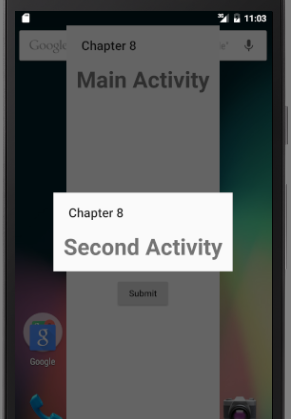
\includegraphics[scale=0.4]{chapters/ch08/images/14}
\end{center}

The interesting thing to note here is that if you look at the logcat messages you will notice that only \texttt{onPause} is called and \texttt{onStop} is NOT called. The reason is that our main activity is partially visible. \texttt{onStop} is only called when the activity gets fully hidden. \\

IMPORTANT: Now open up \texttt{styles.xml}, comment line 9 containing \texttt{<item name="android:windowIsFloating">} tag so that our activities are full-screen again. We need this for our next section:

\begin{center}
	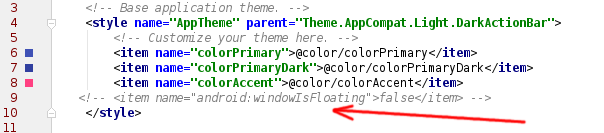
\includegraphics[scale=0.4]{chapters/ch08/images/16}
\end{center}

For a brief official android multi-part tutorial about activity lifecycles please visit \href{https://developer.android.com/training/basics/activity-lifecycle/starting.html}{here}. For more information about activities you can visit \href{https://developer.android.com/guide/components/activities.html}{here}

\subsection{Activity Backstack}

Almost every useful app has many screens that the user can interact with. Every android app maintains something called a \href{https://developer.android.com/guide/components/tasks-and-back-stack.html}{``\texttt{Activity Backstack}''}. As the name implies the backstack is a LIFO (last in first out) data structure. Whenever the user launches an app an empty backstack is created and the launcher activity is pushed onto it. As the user launches another activity then this new activity will be pushed on top of the stack with a fully focused and running state and the previous activity will be pushed one position down the stack in a paused/stopped state. Consider the following diagram (image source: \href{https://developer.android.com/images/fundamentals/diagram_backstack.png}{android docs}):

\begin{center}
	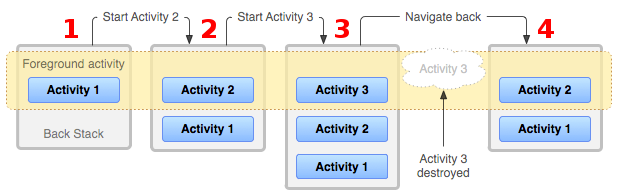
\includegraphics[scale=0.4]{chapters/ch08/images/15}
\end{center}

Let's analyze each stage one by one:

\begin{enumerate}
	\item The user launches the app and the launcher activity called ``Activity 1'' gets pushed on to the backstack. This activity is on top of the stack and is fully active.
	
	\item Now the user starts another activity from activity 1. Let's call the new activity as ``Activity 2''. The activity 2 will be pushed on top of the stack. Activity 1 will be pushed one place down the stack going into a paused/stopped state. ``Activity 2'' will be the currently active activity.
	
	\item ``Activity 3'' is launched from activity 2, pushing activity 2 down one place and in a suspended state. Activity 3 will be the new active activity.
	
	Note that even though activity 1 and 2 are in a suspended state they still reside in the memory and are NOT destroyed.
	
	\item ``Activity 3'' is destroyed e.g: user presses the back button. In this case activity 3 will be pushed off the stack and will be completely removed from the system resources. The activity underneath it (in this case Activity 2) will be made the current top of the stack. Hence activity 2 will be upgraded from paused/stopped state to a resumed and fully active state.
\end{enumerate}

\begin{quote}
	``\textit{\textbf{Definition:}} A collection of activities on a backstack is called a \href{https://developer.android.com/guide/components/tasks-and-back-stack.html#ManagingTasks}{\texttt{Task}}.''
\end{quote}

We will not go into the details of the tasks, just this definition is sufficient for now. For more information about the activity backstack please visit \href{https://developer.android.com/guide/components/tasks-and-back-stack.html}{this link}.
